% Options for packages loaded elsewhere
\PassOptionsToPackage{unicode}{hyperref}
\PassOptionsToPackage{hyphens}{url}
%
\documentclass[
  12pt,
]{article}
\title{El Niño Southern Oscillation Effects in Western Washington}
\usepackage{etoolbox}
\makeatletter
\providecommand{\subtitle}[1]{% add subtitle to \maketitle
  \apptocmd{\@title}{\par {\large #1 \par}}{}{}
}
\makeatother
\subtitle{\url{https://github.com/sashakeller/ElNinoWa}}
\author{Sasha Keller}
\date{}

\usepackage{amsmath,amssymb}
\usepackage{lmodern}
\usepackage{iftex}
\ifPDFTeX
  \usepackage[T1]{fontenc}
  \usepackage[utf8]{inputenc}
  \usepackage{textcomp} % provide euro and other symbols
\else % if luatex or xetex
  \usepackage{unicode-math}
  \defaultfontfeatures{Scale=MatchLowercase}
  \defaultfontfeatures[\rmfamily]{Ligatures=TeX,Scale=1}
  \setmainfont[]{Times New Roman}
\fi
% Use upquote if available, for straight quotes in verbatim environments
\IfFileExists{upquote.sty}{\usepackage{upquote}}{}
\IfFileExists{microtype.sty}{% use microtype if available
  \usepackage[]{microtype}
  \UseMicrotypeSet[protrusion]{basicmath} % disable protrusion for tt fonts
}{}
\makeatletter
\@ifundefined{KOMAClassName}{% if non-KOMA class
  \IfFileExists{parskip.sty}{%
    \usepackage{parskip}
  }{% else
    \setlength{\parindent}{0pt}
    \setlength{\parskip}{6pt plus 2pt minus 1pt}}
}{% if KOMA class
  \KOMAoptions{parskip=half}}
\makeatother
\usepackage{xcolor}
\IfFileExists{xurl.sty}{\usepackage{xurl}}{} % add URL line breaks if available
\IfFileExists{bookmark.sty}{\usepackage{bookmark}}{\usepackage{hyperref}}
\hypersetup{
  pdftitle={El Niño Southern Oscillation Effects in Western Washington},
  pdfauthor={Sasha Keller},
  hidelinks,
  pdfcreator={LaTeX via pandoc}}
\urlstyle{same} % disable monospaced font for URLs
\usepackage[margin=2.54cm]{geometry}
\usepackage{graphicx}
\makeatletter
\def\maxwidth{\ifdim\Gin@nat@width>\linewidth\linewidth\else\Gin@nat@width\fi}
\def\maxheight{\ifdim\Gin@nat@height>\textheight\textheight\else\Gin@nat@height\fi}
\makeatother
% Scale images if necessary, so that they will not overflow the page
% margins by default, and it is still possible to overwrite the defaults
% using explicit options in \includegraphics[width, height, ...]{}
\setkeys{Gin}{width=\maxwidth,height=\maxheight,keepaspectratio}
% Set default figure placement to htbp
\makeatletter
\def\fps@figure{htbp}
\makeatother
\setlength{\emergencystretch}{3em} % prevent overfull lines
\providecommand{\tightlist}{%
  \setlength{\itemsep}{0pt}\setlength{\parskip}{0pt}}
\setcounter{secnumdepth}{5}
\ifLuaTeX
  \usepackage{selnolig}  % disable illegal ligatures
\fi

\begin{document}
\maketitle

\newpage

\hypertarget{rationale-and-research-questions}{%
\section{Rationale and Research
Questions}\label{rationale-and-research-questions}}

As we go out into a new world racked with climate change, we will
encounter shifts in weather patterns with drastic consequences.
Environmental managers must be aware of these alternate regimes and
their potential consequences. To this end I am investigating effects of
El Niño and La Niña on streams in Western Washington state. I will focus
on discharge data to investigate potential effects on water supply under
each of these weather patterns and the absence of them.

Due to the shifting and spontaneous nature of the El-Niño Southern
Oscillation (ENSO) cycle, the data samples are irregular in length and
the data is expected to be skewed depending on the cycle. It is expected
that in the Pacific Northwest El Niño patterns results in drier and
warmer weather, while La Niña should produce wetter and cooler weather
(What are El Niño and La Niña?, 2022). This further prevents the data
from being normally distributed. To overcome these obstacles
non-parametric statistical analyses, namely the Kruskal-Wallis and
Wilcoxon Rank Sum tests, will be employed to identify whether these
climate pressures yield different samples of discharge from a variety of
USGS gages.

\begin{enumerate}
\def\labelenumi{\arabic{enumi}.}
\tightlist
\item
  Do ENSO cycles affect discharge patterns in Western Washington?
\item
  What is the scale of these effects?
\end{enumerate}

\newpage

\hypertarget{dataset-information}{%
\section{Dataset Information}\label{dataset-information}}

Two data sources were required to address the research questions:
discharge data and ENSO data indicating when El Niño and La Niña cycles
were in effect. Discharge data was sourced from USGS Gage data through
the dataRetrieval package. ENSO status was sourced from NOAA and
processed through a script graciously provided by Dr.~Luke Parsons. ENSO
data is measured in Sea Surface Temperature (SST) in degrees Celsius.
Any months with SST above 0.5°C were marked as under an El Niño cycle
and all months below -0.5°C were marked as under a La Niña cycle, as per
NOAA convention.

\newpage

\hypertarget{exploratory-analysis}{%
\section{Exploratory Analysis}\label{exploratory-analysis}}

Visual inspection of discharge data, ENSO cycles, and their overlap
informed my approach to statistical tests and data wrangling. As is
immediately evident in Figure 1, ENSO cycles are not very evenly
distributed. While we can see in Figures 2-4 that discharges among the
four sites are fairly consistent with high discharge event signals
appearing throughout, they do appear to have their own local forces
acting upon them. The highest peak discharge events are unique to each
stream, for example. Each of these peak events also appear to occur in a
La Niña season, but there does not appear to be a glaring high
discharge-low discharge dichotomy based on ENSO cycle. Summary
statistics are shown in Figures 5-9.

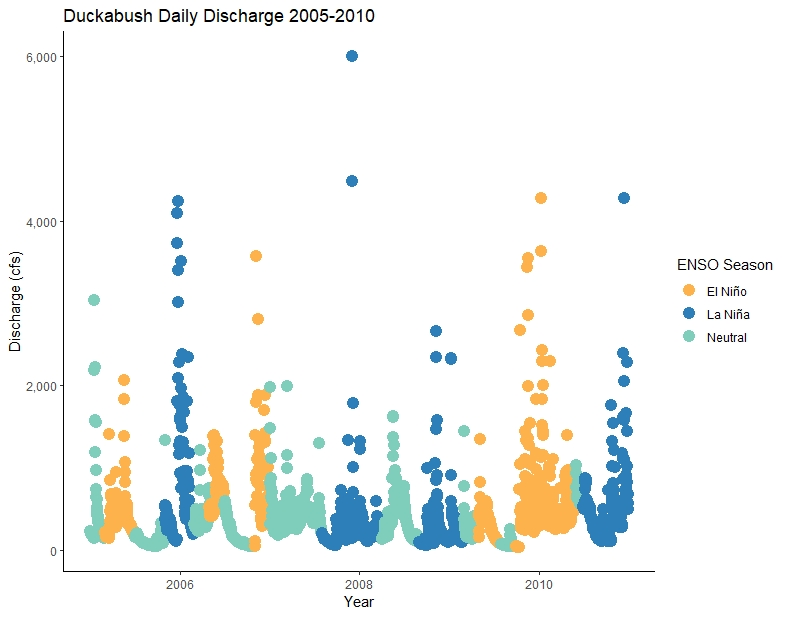
\includegraphics{Data/Processed/ExampleDischarge.jpeg} \textbf{Figure
1}:ENSO Cycles in Duckabush Discharge

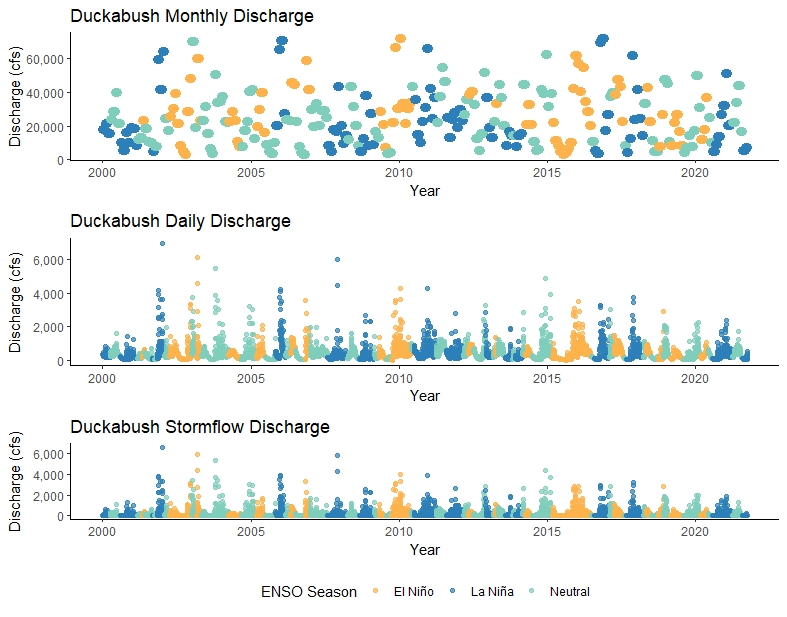
\includegraphics{Data/Processed/Plots/DuckPlots.jpeg} \textbf{Figure
2}:Duckabush Discharge Plots

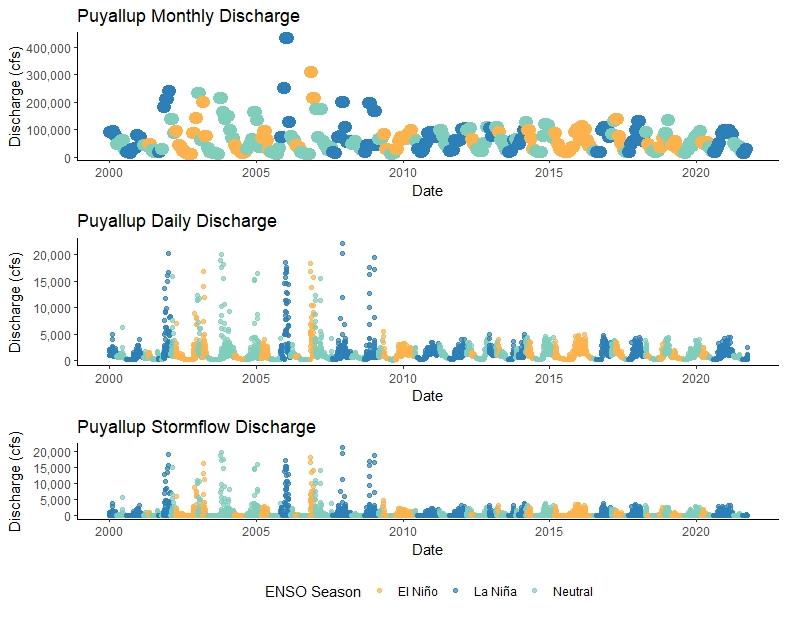
\includegraphics{Data/Processed/Plots/PuyallupPlots.jpeg} \textbf{Figure
3}:Puyallup Discharge Plots

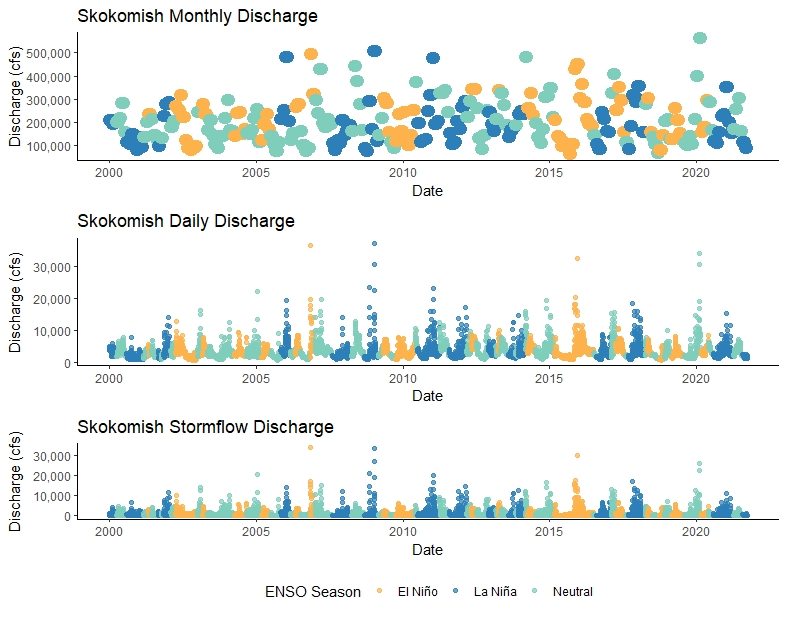
\includegraphics{Data/Processed/Plots/SkokomishPlots.jpeg}
\textbf{Figure 4}:Skokomish Discharge Plots

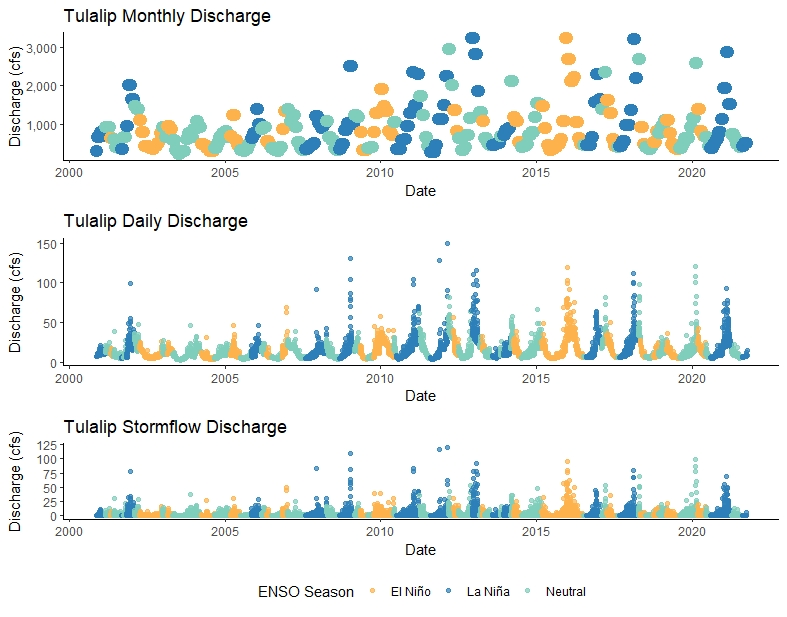
\includegraphics{Data/Processed/Plots/TulalipPlots.jpeg} \textbf{Figure
5}:Tulalip Discharge Plots

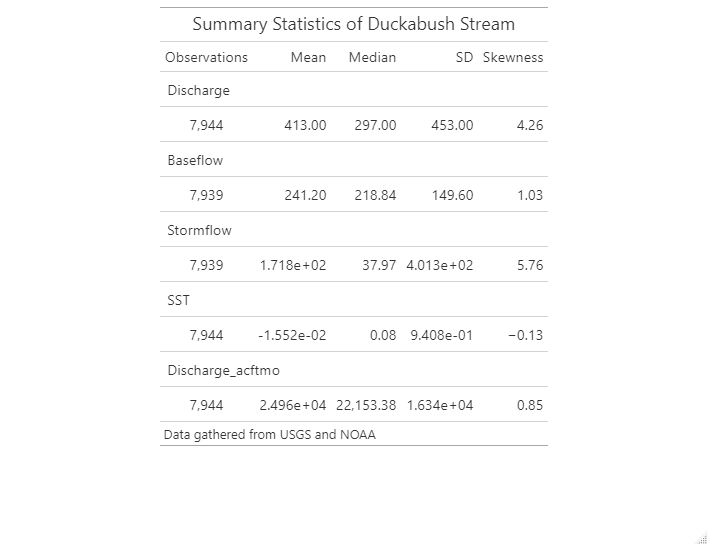
\includegraphics{Data/Processed/SummaryStats/DuckSummStats.jpeg}
\textbf{Figure 6}:Duckabush Summary Statistics

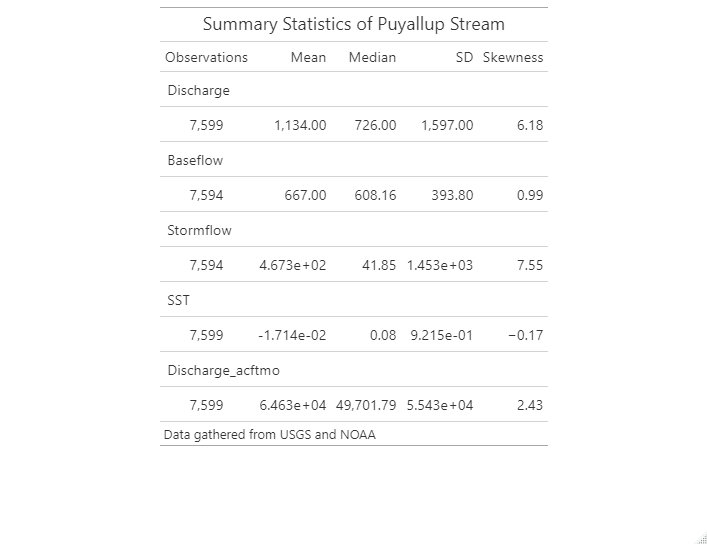
\includegraphics{Data/Processed/SummaryStats/PuyaSummStats.jpeg}
\textbf{Figure 7}:Puyallup Stream Summary Statistics

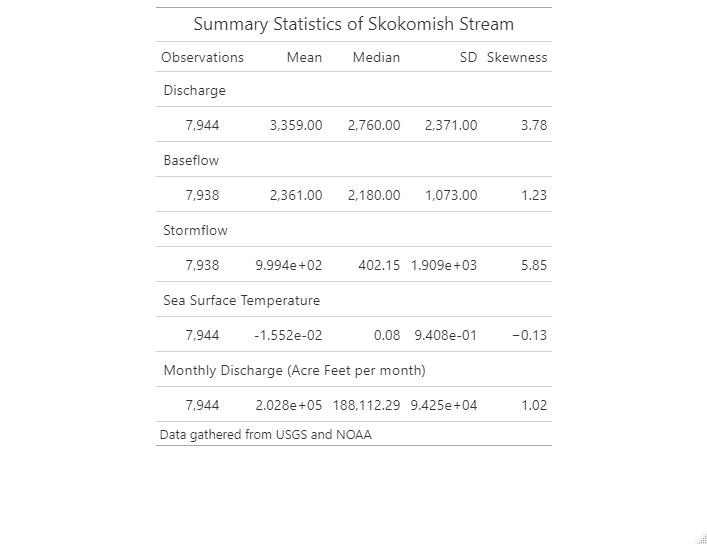
\includegraphics{Data/Processed/SummaryStats/SkokomishSummStats.jpeg}
\textbf{Figure 8}:Skokomish Stream Summary Statistics

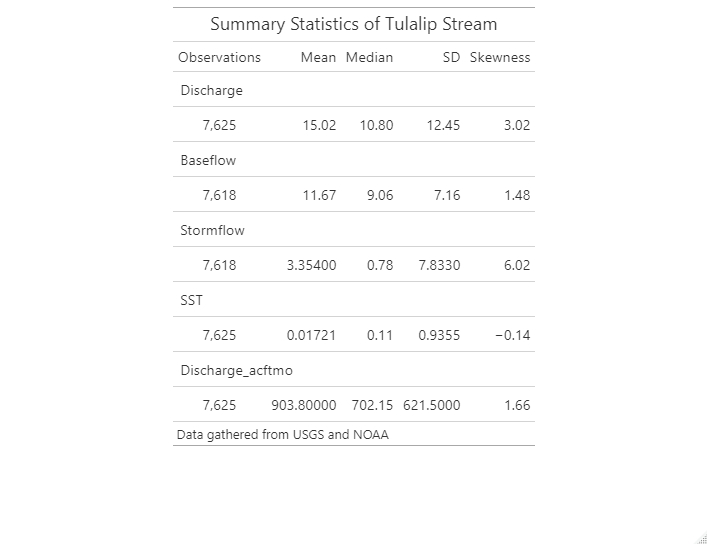
\includegraphics{Data/Processed/SummaryStats/TulaSummStats.jpeg}
\textbf{Figure 9}:Tulalip Stream Summary Statistics

\newpage

\hypertarget{analysis}{%
\section{Analysis}\label{analysis}}

To investigate whether it is possible to identify statistically
significant distinct samples based on ENSO cycles, I employed an initial
Kruskal-Wallis Rank Sum test among all `ENSO Seasons' (El Niño, La Niña,
or Neutral seasons) and then conducted a Wilcoxon Rank Sum test among
each possible pair of seasons. This was repeated for each stream.

\hypertarget{do-enso-cycles-affect-discharge-patterns-in-western-washington}{%
\subsection{Do ENSO cycles affect discharge patterns in Western
Washington?}\label{do-enso-cycles-affect-discharge-patterns-in-western-washington}}

Figure 11 shows the Kruskal-Wallis p value results for each level of
discharge, all of which gave significant results. This indicates a clear
differentiation between discharge samples based on their ENSO season.
They are statistically distinct, but we cannot identify how they are
distinct through this non-parametric test. This provides the impetus to
dig deeper and discover where these effects are accentuated the most.
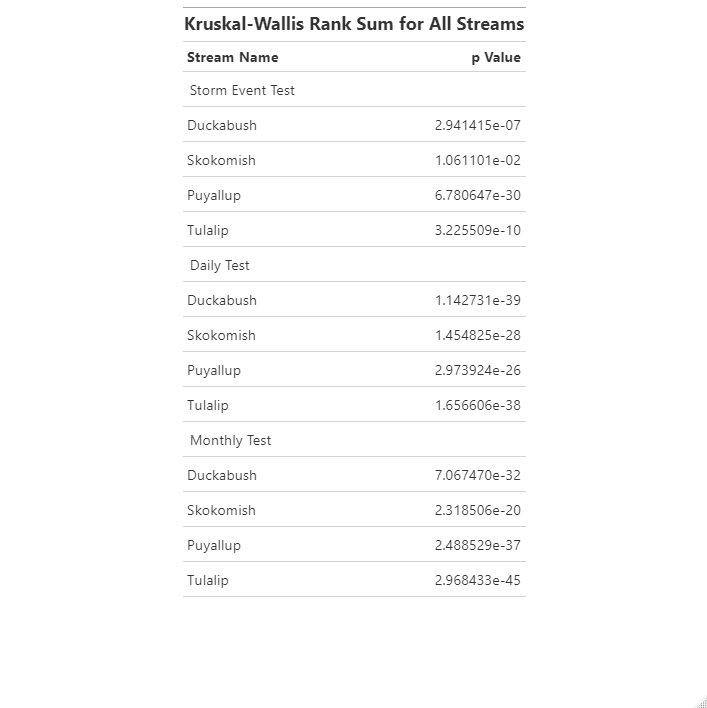
\includegraphics{Data/Processed/Tables/KTTable.jpeg} \textbf{Figure
10}:Kruskal-Wallis Results for All Streams

\hypertarget{what-is-the-scale-of-these-effects}{%
\subsection{What is the scale of these
effects?}\label{what-is-the-scale-of-these-effects}}

Figures 11-14 show the Wilcoxon Rank Sum p values across each pair
comparison for each stream. Almost all of these results identified
statistically significant differences in samples. However, we can
identify three non-significant comparisons: the El Niño and Neutral
sample comparison for the Tulalip, Skokomish, and Puyallup streams among
stormflow discharge. The La Niña-Neutral stormflow comparison for the
Duckabush featured a lower level of significance, but we can note that
the La Niña-El Niño comparison for all streams under stormflow were
highly significant. All of these significant results indicate that
almost every pair tested in each discharge dataset proved to be distinct
from each other. The non-parametric nature of the test does not inform
us which season has higher or lower discharge, only that they are
statistically different from one another.

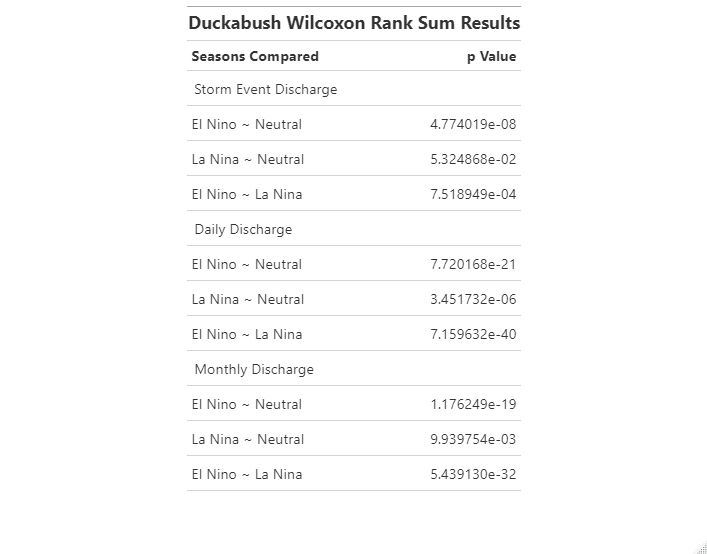
\includegraphics{Data/Processed/Tables/DuckWTTable.jpeg} \textbf{Figure
11}:Duckabush Wilcoxon Test Results

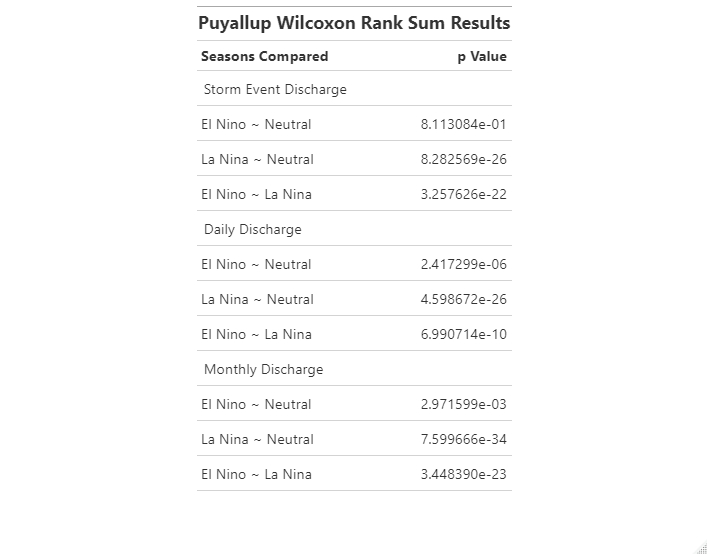
\includegraphics{Data/Processed/Tables/PuyallupWTTable.jpeg}
\textbf{Figure 12}:Puyallup Wilcoxon Test Results

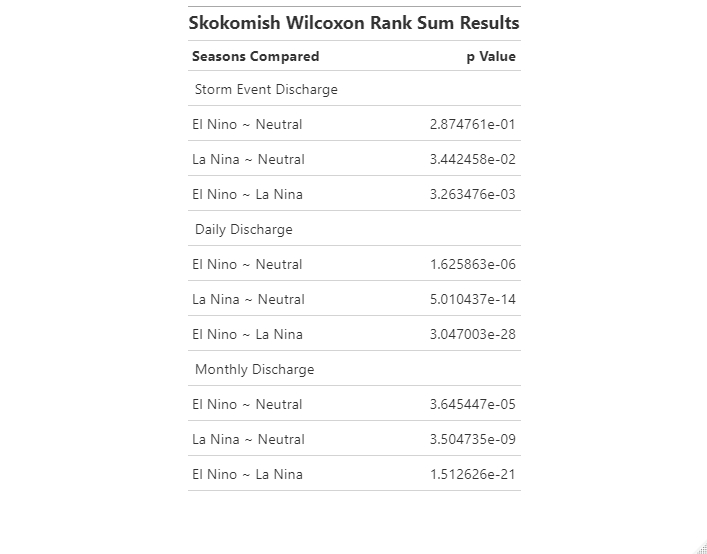
\includegraphics{Data/Processed/Tables/SkoWTtable.jpeg} \textbf{Figure
13}:Skokomish Wilcoxon Test Results

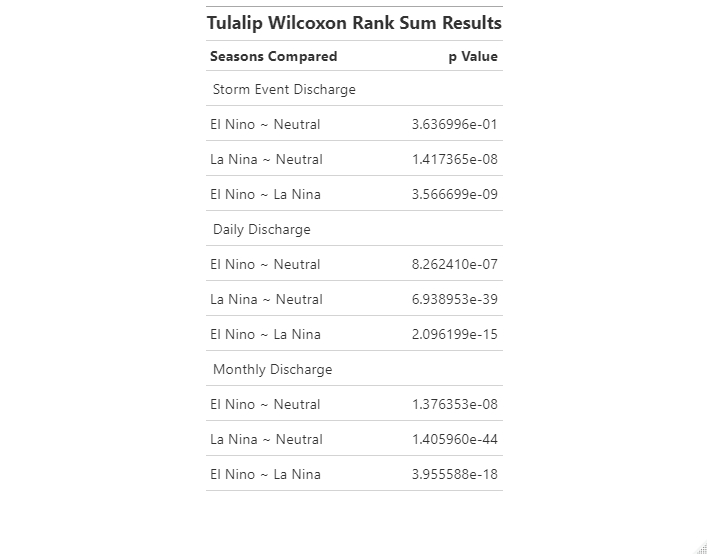
\includegraphics{Data/Processed/Tables/TulaWTTable.jpeg} \textbf{Figure
14}:Tulalip Wilcoxon Test Results

\newpage

\hypertarget{summary-and-conclusions}{%
\section{Summary and Conclusions}\label{summary-and-conclusions}}

In this particular case, a sea of significant results does not tell very
much of a story. It supports the notion that ENSO seasons do affect
discharge and these discharge regimes are unique. It cannot be confirmed
whether it supports NOAA's claim of wetter La Niña seasons and drier El
Niño seasons is true, but it is clear that ENSO cycles are felt in a
variety of different streams. Despite the huge amount of variation in
discharge, and a potential dam installation in the case of the Puyallup,
ENSO cycles retain their significance in distinction. While further
site-specific study is recommended for particular management
recommendations, ENSO cycles are found to be a powerful force across all
study sites. With climate change potentially exacerbating these cycles,
the effects on discharge should remain a topic of interest for managers
across Western Washington.

\newpage

\hypertarget{references}{%
\section{References}\label{references}}

What are El Niño and La Niña? (n.d.). National Ocean Service. Retrieved
April 24, 2022, from
\url{https://oceanservice.noaa.gov/facts/ninonina.html\#}:\textasciitilde:text=Episodes\%20of\%20El\%20Ni\%C3\%B1o\%20and,more\%20frequently\%20than\%20La\%20Ni\%C3\%B1a.

\end{document}
